\documentclass{beamer}
\usepackage[utf8]{inputenc}
\usepackage{textpos} 
\usepackage{graphicx} 
\graphicspath{{./}{DPR_tex/}}
\usepackage{wrapfig}
\usepackage{tikz}
\usetikzlibrary{shapes.geometric,calc, arrows.meta, positioning,fit}
\usepackage{amsmath}
\usepackage{amssymb}
\usepackage[framemethod=TikZ]{mdframed}
\usepackage{caption} 
\usetheme{Boadilla}
\usecolortheme{default}
\usepackage{lmodern}
\usepackage{array}
\usepackage{pgfgantt}
\usepackage{pgf-umlsd}
\usepackage{listings}
\hfuzz=3pt

\tikzstyle{actor} = [draw, ellipse, minimum height=1.5em, minimum width=3em, align=center]
\tikzstyle{usecase} = [draw, ellipse, minimum height=2.5em, text centered]
\setbeamertemplate{caption}[numbered]
\renewcommand{\listfigurename}{Table des figures}
\makeatletter
\@ifundefined{tf@lof}{\newwrite\tf@lof}{}
\immediate\openout\tf@lof=\jobname.lof\relax
\newcommand{\storedfigurelist}{}
\newcommand{\figurelistentry}[3]{%
  \g@addto@macro\storedfigurelist{\noindent \textbf{Figure #1.} #2 \dotfill #3\par}%
}
\newcommand{\recordfigureentry}[1]{%
  \protected@write\@auxout{}{\string\figurelistentry{\thefigure}{#1}{\thepage}}%
}
\newcommand{\dynamiclistoffigures}{%
  \begingroup
  \parindent=0pt
  \parskip=0.35em
  \footnotesize
  \ifx\storedfigurelist\@empty
    \textit{Aucune figure répertoriée pour le moment.}%
  \else
    \storedfigurelist
  \fi
  \endgroup
}
\makeatother

\newcommand{\slidepurpose}[2]{%
\vspace*{-0.23cm}
\begin{center}
{\tiny
\setlength{\fboxsep}{3pt}%
\setlength{\fboxrule}{0.6pt}%
\fcolorbox{black!55}{gray!10}{%
\parbox{\dimexpr0.97\linewidth-2\fboxsep-2\fboxrule\relax}{\raggedright
\textbf{Role :} #1 \hfill \textbf{Etape du projet :} #2}}}
\end{center}
\vspace{0.03cm}
}
\newcommand{\defitem}[2]{\textbf{#1} : #2\par\vspace{0.32em}}
\newcommand{\solutionfigure}[2]{%
\begin{center}
\fcolorbox{blue!60!black}{gray!08}{%
\begin{minipage}[c][0.37\textheight][c]{0.94\linewidth}
\centering
\includegraphics[width=0.9\linewidth,height=0.28\textheight,keepaspectratio]{#1}
\end{minipage}}
\vspace{0.06cm}
{\captionsetup{type=figure,font=tiny,justification=centering}
\captionof{figure}{#2}%
\addcontentsline{lof}{figure}{\protect\numberline{\thefigure}{#2}}%
\recordfigureentry{#2}}
\end{center}
}

\title[Rapport Projet] 
{Présentation PFA: Détection de pneumonie\\sur radiographie}

\subtitle{Conception, Modélisation et Développement.}

\author[HANFAOUI.K et KAFIF.I] 
{HANFAOUI Karim\inst{1} \and KAFIF. Imane\inst{2}}

\institute[EMSI] 
{
  \inst{1} EMSI, 4ème Année IADO G2 - \\
  Karim.Hanfaoui@emsi-edu.ma \\
  \inst{2} EMSI, 4ème Année IADO G2 - \\
  Imane.Kafif@emsi-edu.ma 
}

\date[MAR 2026] 
{EMSI Les Orangers, Mars 2026}
\titlegraphic{
\includegraphics[height=0.7cm]{logo.png}}

\AtBeginSection[]
{
  \begin{frame}
    \frametitle{Table des Matières}
    \slidepurpose{Repérer la section courante et le type de contenu qui suit}{Navigation / structuration}
    \tableofcontents[currentsection]
  \end{frame}
}

\begin{document}

\begin{frame}
    \titlepage
\end{frame}

\begin{frame}
\frametitle{Table des Matières}
\slidepurpose{Présenter la structure complète du rapport et l'ordre des étapes}{Navigation / cadrage global}
\tableofcontents
\end{frame}

\begin{frame}[t]
\frametitle{Table des figures}
\slidepurpose{Référencer automatiquement toutes les figures du document}{Navigation / repérage documentaire}
\dynamiclistoffigures
\end{frame}

\section{Acronymes et terminologie}
\subsection{Glossaire initial}

\begin{frame}{Acronymes — Domaine et modèles}
\slidepurpose{Donner les sigles du domaine avant les slides techniques}{Référence documentaire}
\small
\begin{columns}[T,onlytextwidth]
\begin{column}{0.48\textwidth}
\begin{block}{Domaine médical et IA}
\defitem{IA}{Intelligence Artificielle.}
\defitem{DL}{Deep Learning, famille de modèles à plusieurs couches.}
\defitem{CXR}{Chest X-Ray, radiographie thoracique.}
\defitem{SOTA}{State Of The Art, meilleur niveau connu au moment de l'étude.}
\end{block}
\end{column}
\begin{column}{0.48\textwidth}
\begin{block}{Modèles et approches}
\defitem{CNN}{Convolutional Neural Network, réseau fondé sur les convolutions.}
\defitem{ViT}{Vision Transformer, adaptation du Transformer aux images.}
\defitem{Swin}{Shifted Window Transformer, Transformer hiérarchique à fenêtres décalées.}
\defitem{Grad-CAM}{Gradient-weighted Class Activation Mapping, outil d'explicabilité visuelle.}
\end{block}
\end{column}
\end{columns}
\end{frame}

\begin{frame}{Acronymes — Blocs techniques}
\slidepurpose{Définir les sigles techniques utilisés dans les architectures et l'évaluation}{Référence documentaire}
\small
\begin{columns}[T,onlytextwidth]
\begin{column}{0.48\textwidth}
\begin{block}{Architecture}
\defitem{BN}{Batch Normalization, normalisation des activations sur un mini-batch.}
\defitem{ReLU}{Rectified Linear Unit, activation $f(x)=\max(0,x)$.}
\defitem{GAP}{Global Average Pooling, moyenne spatiale par canal.}
\defitem{FC}{Fully Connected, couche dense finale de décision.}
\end{block}
\end{column}
\begin{column}{0.48\textwidth}
\begin{block}{Efficacité et confiance}
\defitem{MBConv}{Mobile Inverted Bottleneck Convolution, bloc compact d'EfficientNet.}
\defitem{SE}{Squeeze-and-Excitation, mécanisme de ré-pondération des canaux.}
\defitem{FLOPs}{Floating Point Operations, estimation du coût de calcul.}
\defitem{ECE}{Expected Calibration Error, mesure de calibration des probabilités.}
\end{block}
\end{column}
\end{columns}
\end{frame}

\begin{frame}{Notations mathématiques}
\slidepurpose{Définir les notations qui reviennent dans les équations et les schémas}{Référence documentaire}
\small
\begin{columns}[T,onlytextwidth]
\begin{column}{0.48\textwidth}
\begin{block}{Tailles et dimensions}
\defitem{$H,W$}{Hauteur et largeur spatiales d'une image ou d'une carte de features.}
\defitem{$C$}{Nombre de canaux.}
\defitem{$L$}{Nombre de couches ou de blocs, selon le contexte.}
\defitem{$k$}{Growth rate DenseNet, nombre de nouveaux canaux ajoutés par couche.}
\end{block}
\end{column}
\begin{column}{0.48\textwidth}
\begin{block}{Variables de modélisation}
\defitem{$\phi$}{Facteur global de scaling dans EfficientNet.}
\defitem{$X$}{Image d'entrée.}
\defitem{$F$}{Tensor de features appris par le modèle.}
\defitem{$p(y|X)$}{Probabilité prédite pour une classe $y$ conditionnée par l'image $X$.}
\end{block}
\end{column}
\end{columns}
\end{frame}

\begin{frame}{Terminologie d'architecture}
\slidepurpose{Définir les termes techniques utilisés sans alourdir les slides principales}{Référence documentaire}
\small
\begin{columns}[T,onlytextwidth]
\begin{column}{0.48\textwidth}
\begin{block}{CNN et représentations}
\defitem{Feature map}{Carte d'activation produite par un bloc du réseau.}
\defitem{Backbone}{Extracteur principal de représentations d'une architecture.}
\defitem{Bottleneck}{Réduction intermédiaire des canaux pour baisser le coût.}
\defitem{Skip connection}{Chemin de contournement transmettant une information plus tôt dans le réseau.}
\end{block}
\end{column}
\begin{column}{0.48\textwidth}
\begin{block}{Transformers et fiabilité}
\defitem{Token}{Unité d'entrée d'un Transformer, ici un patch projeté.}
\defitem{Embedding}{Représentation vectorielle dense d'un objet discret ou local.}
\defitem{Calibration}{Adéquation entre probabilité annoncée et fréquence réelle de succès.}
\defitem{Heatmap}{Carte colorée montrant des zones activées ou importantes pour la décision.}
\end{block}
\end{column}
\end{columns}
\end{frame}

\begin{frame}{Guide de lecture du document}
\slidepurpose{Préciser le rôle exact de chaque groupe de slides dans la fabrication du projet}{Lecture guidée du rapport}
\small
\begin{columns}[T,onlytextwidth]
\begin{column}{0.48\textwidth}
\begin{block}{Cadrage}
\defitem{Problématique / Méthodologie}{Définir le besoin clinique, la question scientifique et l'organisation du travail.}
\defitem{Analyse SOTA}{Comparer les approches existantes avant de choisir une direction.}
\end{block}
\begin{block}{Conception}
\defitem{Solution proposée}{Définir l'architecture cible, sa logique et ses sorties.}
\end{block}
\end{column}
\begin{column}{0.48\textwidth}
\begin{block}{Validation}
\defitem{Résultats}{Mesurer la performance finale et lire les indicateurs.}
\defitem{Annexes}{Documenter les notions techniques non développées dans le flux principal.}
\end{block}
\begin{block}{Principe de lecture}
Chaque slide technique indique explicitement :
\begin{itemize}
\setlength{\itemsep}{0.3em}
\item son \textbf{role} dans le document,
\item l'\textbf{etape du projet} à laquelle il appartient.
\end{itemize}
\end{block}
\end{column}
\end{columns}
\end{frame}

\section{Problématique et Méthodologie}

\begin{frame}{Problématique}
\slidepurpose{Poser le besoin clinique, la question de recherche et la contrainte d'explicabilité}{Cadrage scientifique}
    \begin{alertblock}{Question Centrale de Recherche}
        Face à la complexité visuelle des pathologies pulmonaires et à la pénurie mondiale de radiologues experts, comment pouvons-nous concevoir un système automatisé basé sur le Deep Learning capable non seulement de détecter la pneumonie avec une précision clinique supérieure à l'interprétation humaine, mais aussi de fournir une justification visuelle explicable afin de garantir une intégration sécurisée et fiable dans le flux de travail médical d'urgence ?
    \end{alertblock}
\end{frame}

\begin{frame}{Méthodologie : Approche Agile (Scrum)}
\slidepurpose{Montrer comment le projet est découpé en phases de travail et d'itération}{Organisation / planification}
    \centering
    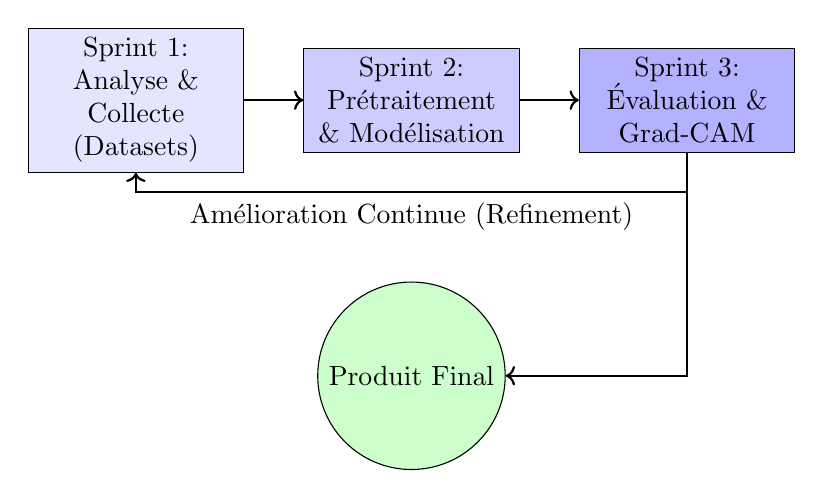
\begin{tikzpicture}[node distance=2cm, auto]
        \node[draw, rectangle, fill=blue!10, text width=2.5cm, align=center] (sprint1) {Sprint 1:\\Analyse \& Collecte (Datasets)};
        \node[draw, rectangle, fill=blue!20, text width=2.5cm, align=center, right of=sprint1, xshift=1.5cm] (sprint2) {Sprint 2:\\Prétraitement \& Modélisation};
        \node[draw, rectangle, fill=blue!30, text width=2.5cm, align=center, right of=sprint2, xshift=1.5cm] (sprint3) {Sprint 3:\\Évaluation \& Grad-CAM};
        
        \draw[thick, ->] (sprint1) -- (sprint2);
        \draw[thick, ->] (sprint2) -- (sprint3);
        \draw[thick, ->] (sprint3.south) |- ++(0,-0.5) -| (sprint1.south) node[pos=0.25, below] {Amélioration Continue (Refinement)};
        
        \node[draw, circle, fill=green!20, below of=sprint2, yshift=-1.5cm] (delivery) {Produit Final};
        \draw[thick, ->] (sprint3) |- (delivery);
    \end{tikzpicture}
    \begin{itemize}
        \item \textbf{Flexibilité :} Adaptation aux contraintes des données médicales.
        \item \textbf{Itérations :} Optimisation progressive des hyperparamètres.
    \end{itemize}
\end{frame}

\section{Analyse SOTA}
\subsection{Phase 1 — DenseNet / CheXNet}

\begin{frame}{SOTA : Architecture DenseNet-121}
\slidepurpose{Présenter le modele CNN de référence utilisé comme base de comparaison}{Analyse SOTA / comparaison}
\vspace*{-0.35cm}
\centering
\resizebox{0.95\textwidth}{!}{%
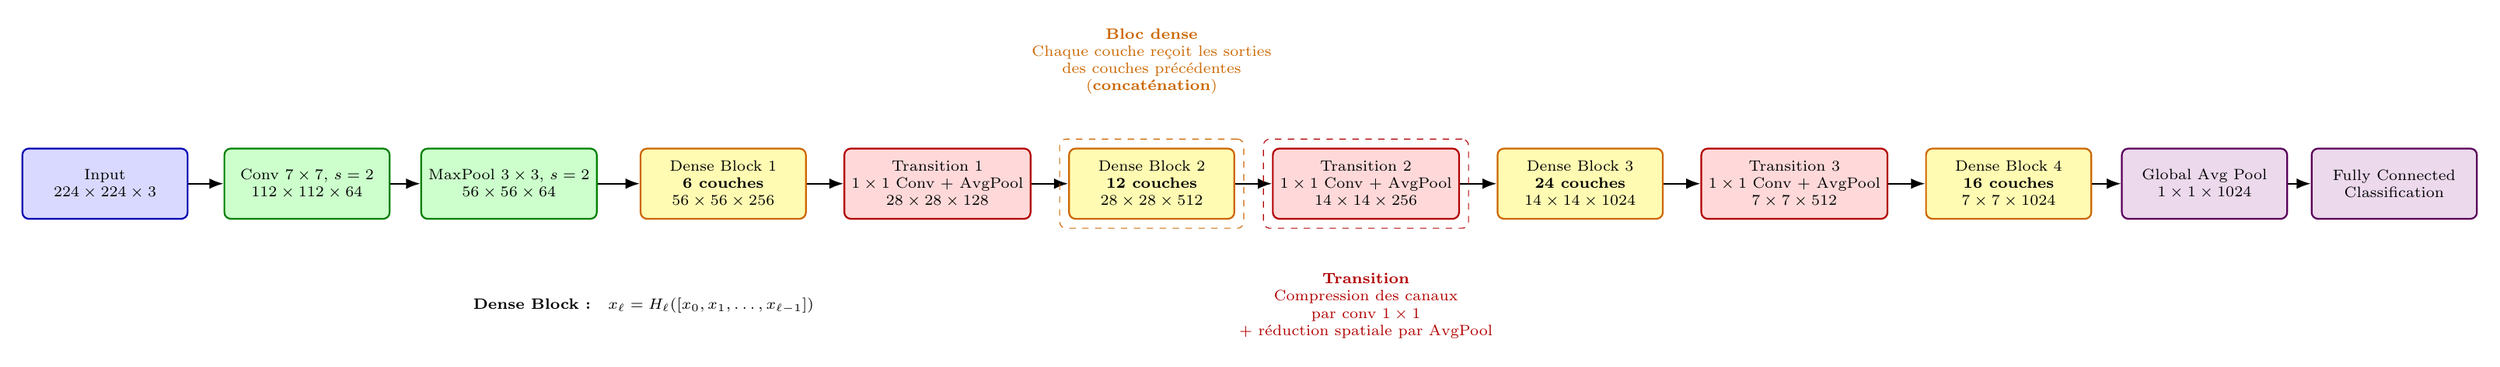
\begin{tikzpicture}[
    >=Latex,
    font=\scriptsize,
    op/.style={
        draw,
        rounded corners=3pt,
        minimum width=2.7cm,
        minimum height=1.15cm,
        align=center,
        thick
    },
    io/.style={op, fill=blue!15, draw=blue!70!black},
    stem/.style={op, fill=green!20, draw=green!50!black},
    dense/.style={op, fill=yellow!30, draw=orange!80!black},
    trans/.style={op, fill=red!15, draw=red!70!black},
    head/.style={op, fill=violet!15, draw=violet!70!black},
    explain/.style={draw, dashed, rounded corners=3pt, inner sep=4pt}
]

% ligne principale
\node[io]    (in)   at (0,0)    {Input\\$224\times224\times3$};
\node[stem]  (c1)   at (3.3,0)  {Conv $7\times7$, $s=2$\\$112\times112\times64$};
\node[stem]  (mp)   at (6.6,0)  {MaxPool $3\times3$, $s=2$\\$56\times56\times64$};
\node[dense] (db1)  at (10.1,0) {Dense Block 1\\\textbf{6 couches}\\$56\times56\times256$};
\node[trans] (tr1)  at (13.6,0) {Transition 1\\$1\times1$ Conv + AvgPool\\$28\times28\times128$};
\node[dense] (db2)  at (17.1,0) {Dense Block 2\\\textbf{12 couches}\\$28\times28\times512$};
\node[trans] (tr2)  at (20.6,0) {Transition 2\\$1\times1$ Conv + AvgPool\\$14\times14\times256$};
\node[dense] (db3)  at (24.1,0) {Dense Block 3\\\textbf{24 couches}\\$14\times14\times1024$};
\node[trans] (tr3)  at (27.6,0) {Transition 3\\$1\times1$ Conv + AvgPool\\$7\times7\times512$};
\node[dense] (db4)  at (31.1,0) {Dense Block 4\\\textbf{16 couches}\\$7\times7\times1024$};
\node[head]  (gap)  at (34.3,0) {Global Avg Pool\\$1\times1\times1024$};
\node[head]  (fc)   at (37.4,0) {Fully Connected\\Classification};

% flèches
\draw[->, thick] (in)  -- (c1);
\draw[->, thick] (c1)  -- (mp);
\draw[->, thick] (mp)  -- (db1);
\draw[->, thick] (db1) -- (tr1);
\draw[->, thick] (tr1) -- (db2);
\draw[->, thick] (db2) -- (tr2);
\draw[->, thick] (tr2) -- (db3);
\draw[->, thick] (db3) -- (tr3);
\draw[->, thick] (tr3) -- (db4);
\draw[->, thick] (db4) -- (gap);
\draw[->, thick] (gap) -- (fc);

% annotation dense block
\node[explain, draw=orange!80!black, fit=(db2)] {};
\node[align=center, text=orange!80!black] at (17.1,2.0)
{\textbf{Bloc dense}\\Chaque couche reçoit les sorties\\des couches précédentes\\(\textbf{concaténation})};

% annotation transition
\node[explain, draw=red!70!black, fit=(tr2)] {};
\node[align=center, text=red!70!black] at (20.6,-2.0)
{\textbf{Transition}\\Compression des canaux\\par conv $1\times1$\\+ réduction spatiale par AvgPool};

% formule
\node[align=center] at (8.8,-2.0)
{\textbf{Dense Block :}\quad $x_\ell = H_\ell([x_0,x_1,\dots,x_{\ell-1}])$};

\end{tikzpicture}%
}

\vspace{0.01cm}
{\tiny
\setlength{\fboxsep}{3pt}
\setlength{\fboxrule}{0.7pt}
\begin{center}
\begin{minipage}[t]{0.48\textwidth}
\fcolorbox{orange!80!black}{yellow!25}{%
\parbox[t]{\dimexpr\linewidth-2\fboxsep-2\fboxrule-8pt\relax}{\raggedright
\textbf{Dense Block}\\
Concaténation de toutes les cartes précédentes :\\
$x_\ell = H_\ell([x_0,x_1,\dots,x_{\ell-1}])$\\
Réutilisation des features + meilleur flux de gradient.\\
Croissance des canaux : $C_{\text{out}} = C_0 + L\cdot k$.\\
Exemple : $k=32$, $L=6$ $\Rightarrow C_{\text{out}}=C_0+192$.\\
Où $C_0$ = canaux initiaux, $L$ = nb de couches, $k$ = growth rate.
}}
\end{minipage}
\hfill
\begin{minipage}[t]{0.48\textwidth}
\fcolorbox{red!70!black}{red!15}{%
\parbox[t]{\dimexpr\linewidth-2\fboxsep-2\fboxrule\relax}{\raggedright
\textbf{Transition}\\
Entre blocs denses, compresse et réduit.\\
$X\in\mathbb{R}^{H\times W\times C}$\\
$\rightarrow \mathrm{Conv}_{1\times1}(X)=Y\in\mathbb{R}^{H\times W\times C'}$\\
$Y_{h,w,c'}=\sum_{c}W_{c',c}X_{h,w,c}+b_{c'}$\\
$\rightarrow \mathrm{AvgPool}(Y)=Z\in\mathbb{R}^{H/2\times W/2\times C'}$\\
$Z_{i,j,c'}=\tfrac{1}{4}\!\!\sum_{u,v\in\{0,1\}}\!Y_{2i+u,2j+v,c'}$\\
Compression, efficacité, préparation du bloc suivant.\\
Où $H,W$ = hauteur/largeur, $C$ = canaux, $C'$ = canaux compressés.
}}
\end{minipage}

\vspace{0.18cm}

\begin{minipage}[t]{0.48\textwidth}
\fcolorbox{green!50!black}{blue!10}{%
\parbox[t]{\dimexpr\linewidth-2\fboxsep-2\fboxrule\relax}{\raggedright
\textbf{Stem / Entrée}\\
Entrée $224\times224\times3$.\\
Conv $7\times7$ ($s=2$) puis MaxPool $3\times3$ ($s=2$).\\
Extrait des bords/textures et réduit tôt la résolution.\\
Exemple : $224\!\times\!224 \rightarrow 112\!\times\!112 \rightarrow 56\!\times\!56$.\\
Où $H,W$ = dimensions spatiales, $s$ = stride.
}}
\end{minipage}
\hfill
\begin{minipage}[t]{0.48\textwidth}
\fcolorbox{violet!70!black}{violet!15}{%
\parbox[t]{\dimexpr\linewidth-2\fboxsep-2\fboxrule\relax}{\raggedright
\textbf{Tête de classification}\\
Global Avg Pooling : moyenne spatiale par canal.\\
$7\times7\times1024 \rightarrow 1\times1\times1024$.\\
$g_c=\frac{1}{HW}\sum_{h,w}F_{h,w,c}$, puis FC.\\
Exemple : $g\in\mathbb{R}^{1024}\rightarrow \text{scores} \in \mathbb{R}^K$.\\
Où $F$ = carte de features, $g$ = vecteur global, $K$ = nb de classes.
}}
\end{minipage}
\end{center}
}
\end{frame}

\begin{frame}{DenseNet-121 : Structure d'une couche dense}
\slidepurpose{Expliquer le calcul interne d'une couche dense pour comprendre le baseline choisi}{Analyse SOTA / compréhension mécanistique}
\vspace*{-0.2cm}
\begin{columns}[T,onlytextwidth]
\begin{column}{0.46\textwidth}
\centering
\resizebox{\linewidth}{!}{%
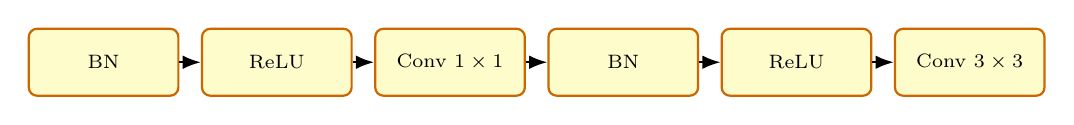
\begin{tikzpicture}[
    >=Latex,
    font=\scriptsize,
    box/.style={
        draw,
        rounded corners=3pt,
        minimum width=1.9cm,
        minimum height=0.85cm,
        align=center,
        thick,
        fill=yellow!20,
        draw=orange!80!black
    }
]
\node[box] (bn1) at (0,0) {BN};
\node[box] (relu1) at (2.2,0) {ReLU};
\node[box] (c11) at (4.4,0) {Conv $1\times1$};
\node[box] (bn2) at (6.6,0) {BN};
\node[box] (relu2) at (8.8,0) {ReLU};
\node[box] (c33) at (11.0,0) {Conv $3\times3$};

\draw[->, thick] (bn1) -- (relu1);
\draw[->, thick] (relu1) -- (c11);
\draw[->, thick] (c11) -- (bn2);
\draw[->, thick] (bn2) -- (relu2);
\draw[->, thick] (relu2) -- (c33);
\end{tikzpicture}
}

\vspace{0.2cm}
{\scriptsize
\parbox{0.9\linewidth}{\centering
\textbf{Séquence :} BN $\rightarrow$ ReLU $\rightarrow$ Conv $1\times1$\\
$\rightarrow$ BN $\rightarrow$ ReLU $\rightarrow$ Conv $3\times3$}
}
\end{column}
\begin{column}{0.54\textwidth}
{\scriptsize
\setlength{\fboxsep}{4pt}
\setlength{\fboxrule}{0.8pt}
\fcolorbox{orange!80!black}{yellow!12}{%
\parbox[t]{\dimexpr\linewidth-2\fboxsep-2\fboxrule\relax}{\raggedright
\textbf{Transformation $H_\ell$}\\
$H_\ell$ est la transformation appliquée par la couche $\ell$ dans un bloc dense ; elle produit de \textbf{nouvelles} cartes de features.\\
\textbf{Formule :}\\
\resizebox{\linewidth}{!}{$H_\ell(x)=\mathrm{Conv}_{3\times3}\big(\mathrm{ReLU}(\mathrm{BN}(\mathrm{Conv}_{1\times1}(\mathrm{ReLU}(\mathrm{BN}(x))))))\big)$}\\
Si $x=[x_0,x_1,\dots,x_{\ell-1}]$, alors $x_\ell=H_\ell(x)$.\\
\textbf{Interprétation :} $1\times1$ = mélange/réduction des canaux (bottleneck),\\
$3\times3$ = extraction spatiale locale, BN+ReLU = stabilité + non-linéarité.\\
\textbf{Croissance :} la couche ajoute $k$ canaux : $C_{\text{out}}=C_{\text{in}}+k$.\\
Après $L$ couches : $C_{\text{out}}=C_0+Lk$.\\
Où $C_{\text{in}}$ = canaux d'entrée, $C_0$ = canaux initiaux, $k$ = growth rate.
}}
}
\end{column}
\end{columns}
\end{frame}

% ==================================================
% PHASE 2 — Optimisation et Efficacité
% ==================================================
\subsection{Phase 2 — Optimisation et efficacité}

\begin{frame}{Phase 2 — EfficientNet : idée générale et scaling}
\slidepurpose{Comparer une stratégie d'optimisation du coût de calcul par scaling équilibré}{Analyse SOTA / comparaison}
\vspace*{-0.2cm}
\begin{columns}[T,onlytextwidth]
\begin{column}{0.52\textwidth}
\centering
\resizebox{\linewidth}{!}{%
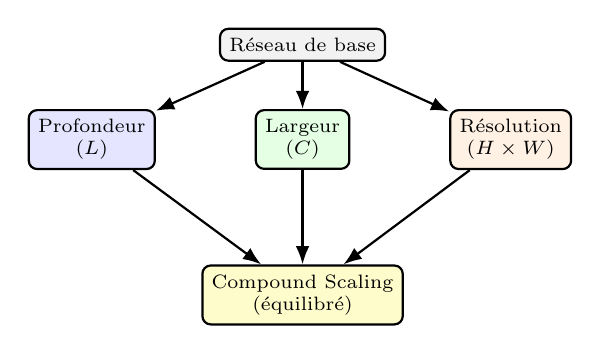
\begin{tikzpicture}[
    >=Latex,
    font=\scriptsize,
    box/.style={draw, rounded corners=3pt, align=center, thick}
]
\node[box, fill=gray!10] (base) {Réseau de base};
\node[box, fill=blue!10, below left=0.6cm and 0.8cm of base] (depth) {Profondeur\\($L$)};
\node[box, fill=green!10, below=0.6cm of base] (width) {Largeur\\($C$)};
\node[box, fill=orange!10, below right=0.6cm and 0.8cm of base] (res) {Résolution\\($H\times W$)};
\node[box, fill=yellow!20, below=1.2cm of width] (compound) {Compound Scaling\\(équilibré)};
\draw[->, thick] (base) -- (depth);
\draw[->, thick] (base) -- (width);
\draw[->, thick] (base) -- (res);
\draw[->, thick] (depth) -- (compound);
\draw[->, thick] (width) -- (compound);
\draw[->, thick] (res) -- (compound);
\end{tikzpicture}
}
\end{column}

\begin{column}{0.48\textwidth}
{\scriptsize
\setlength{\fboxsep}{4pt}
\setlength{\fboxrule}{0.8pt}
\fcolorbox{blue!70!black}{blue!10}{%
\parbox[t]{\dimexpr\linewidth-2\fboxsep-2\fboxrule\relax}{\raggedright
\textbf{Idée centrale}\\
EfficientNet est une famille de CNN conçue pour \textbf{mieux exploiter} un budget de calcul donné.\\
Le \textbf{scaling naïf} (uniquement profondeur, largeur ou résolution) crée un déséquilibre :\\
trop profond $\Rightarrow$ gradient fragile,\\
trop large $\Rightarrow$ surcoût mémoire,\\
trop haute résolution $\Rightarrow$ coût quadratique.
}}
\vspace{0.15cm}
\fcolorbox{green!60!black}{green!10}{%
\parbox[t]{\dimexpr\linewidth-2\fboxsep-2\fboxrule\relax}{\raggedright
\textbf{Compound Scaling}\\
On augmente \textbf{ensemble} profondeur, largeur et résolution par un facteur global $\phi$ pour rester efficace.
}}
}
\end{column}
\end{columns}

\vspace{0.12cm}
\begin{center}
{\scriptsize
\[
\begin{aligned}
d&=\alpha^{\phi},\quad w=\beta^{\phi},\quad r=\gamma^{\phi},\\
\alpha\,\beta^2\,\gamma^2 &\approx 2
\end{aligned}
\]
$\phi$ contrôle l’échelle globale ; la contrainte équilibre coût et performance.
}
\end{center}
\end{frame}

{\hfuzz=5pt\hbadness=10000
\begin{frame}{Phase 2 — MBConv : bloc clé d’EfficientNet}
\slidepurpose{Détailler le bloc opératoire central qui rend EfficientNet efficace}{Analyse SOTA / modélisation d'un bloc}
\vspace*{-0.2cm}
\centering
\resizebox{\textwidth}{!}{%
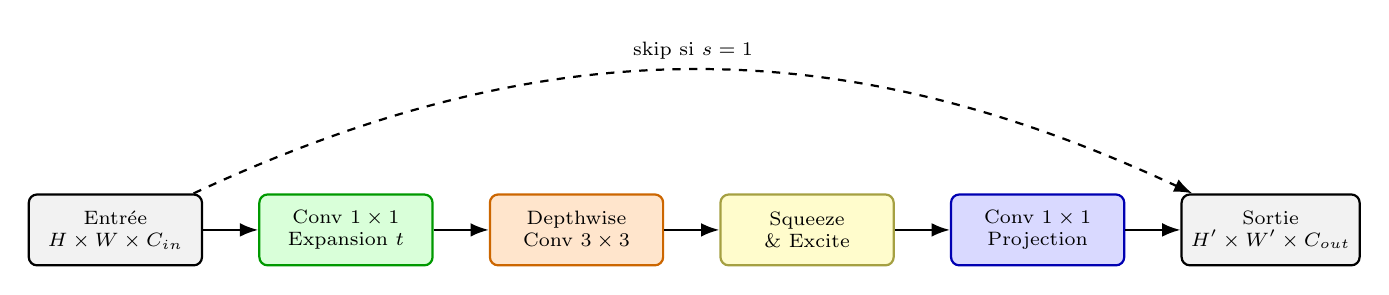
\begin{tikzpicture}[
    >=Latex,
    font=\scriptsize,
    box/.style={draw, rounded corners=3pt, align=center, thick, minimum width=2.2cm, minimum height=0.9cm},
    exp/.style={box, fill=green!15, draw=green!60!black},
    dw/.style={box, fill=orange!20, draw=orange!80!black},
    se/.style={box, fill=yellow!20, draw=yellow!60!black},
    proj/.style={box, fill=blue!15, draw=blue!70!black}
]
\node[box, fill=gray!10] (in) {Entrée\\$H\times W\times C_{in}$};
\node[exp, right=0.7cm of in] (exp) {Conv $1\times1$\\Expansion $t$};
\node[dw, right=0.7cm of exp] (dw) {Depthwise\\Conv $3\times3$};
\node[se, right=0.7cm of dw] (se) {Squeeze\\\& Excite};
\node[proj, right=0.7cm of se] (proj) {Conv $1\times1$\\Projection};
\node[box, fill=gray!10, right=0.7cm of proj] (out) {Sortie\\$H'\times W'\times C_{out}$};

\draw[->, thick] (in) -- (exp);
\draw[->, thick] (exp) -- (dw);
\draw[->, thick] (dw) -- (se);
\draw[->, thick] (se) -- (proj);
\draw[->, thick] (proj) -- (out);

\draw[->, thick, dashed] (in) to[bend left=25] node[above]{skip si $s=1$} (out);
\end{tikzpicture}
}

\vspace{0.12cm}
\begin{columns}[T,onlytextwidth]
\begin{column}{0.5\textwidth}
{\scriptsize
\setlength{\fboxsep}{4pt}
\setlength{\fboxrule}{0.8pt}
\fcolorbox{orange!80!black}{yellow!15}{%
\parbox[t]{\dimexpr\linewidth-2\fboxsep-2\fboxrule\relax}{\raggedright
\textbf{Depthwise Convolution}\\
Chaque canal est filtré séparément :\\
\resizebox{0.6\linewidth}{!}{$Y_{h,w,c}=\sum_{i,j}K^{(c)}_{i,j}\,X_{h+i,w+j,c}$}\\
Coût paramétrique : $k^2 C$\\
au lieu de $k^2 C C'$ (conv standard).\\
Réduit fortement les paramètres et FLOPs.
}}
}
\end{column}
\begin{column}{0.5\textwidth}
{\scriptsize
\fcolorbox{green!60!black}{green!10}{%
\parbox[t]{\dimexpr\linewidth-2\fboxsep-2\fboxrule\relax}{\raggedright
\textbf{MBConv en pratique}\\
1) Expansion\\
$C_e=t\cdot C_{in}$,\\
2) Depthwise $3\times3$,\\
3) SE (ré-pondération canal),\\
4) Projection vers $C_{out}$,\\
5) Skip si stride $s=1$\\
et dimensions\\
compatibles.\\
Objectif :\\
expressivité élevée\\
avec coût réduit.
}}
}
\end{column}
\end{columns}
\end{frame}
}

\begin{frame}{Phase 2 — EfficientNetV2 et impact médical}
\slidepurpose{Montrer l'évolution d'EfficientNet vers une version plus rapide à entraîner et à déployer}{Analyse SOTA / comparaison}
\vspace*{-0.2cm}
\begin{columns}[T,onlytextwidth]
\begin{column}{0.55\textwidth}
{\scriptsize
\setlength{\fboxsep}{4pt}
\setlength{\fboxrule}{0.8pt}
\fcolorbox{blue!70!black}{blue!10}{%
\parbox[t]{\dimexpr\linewidth-2\fboxsep-2\fboxrule\relax}{\raggedright
\textbf{EfficientNetV2 : améliorations}\\
Optimise l’entraînement (plus rapide et stable) via :\\
- \textbf{Fused-MBConv} sur les petits étages (meilleur débit GPU),\\
- règles de scaling adaptées,\\
- stratégies de régularisation plus efficaces.\\
Résultat : \textbf{meilleure précision} à coût d’entraînement réduit.
}}
\vspace{0.15cm}
\fcolorbox{green!60!black}{green!10}{%
\parbox[t]{\dimexpr\linewidth-2\fboxsep-2\fboxrule\relax}{\raggedright
\textbf{Intérêt en imagerie médicale}\\
Meilleur compromis précision/temps :\\
- utile pour stations avec GPU limités,\\
- facilite l’expérimentation rapide,\\
- déploiement clinique plus réaliste.
}}
}
\end{column}
\begin{column}{0.45\textwidth}
\centering
\resizebox{\linewidth}{!}{%
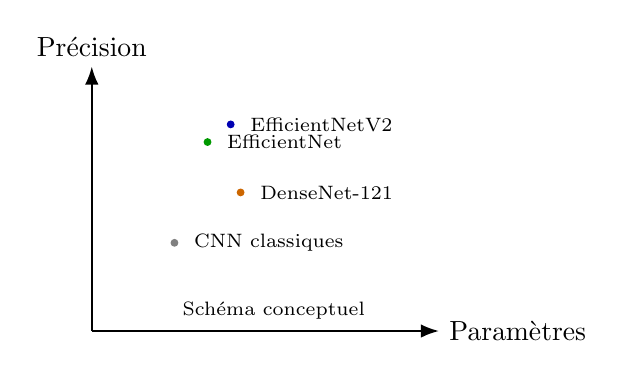
\begin{tikzpicture}[x=4.2cm,y=3.2cm,>=Latex]
\draw[->, thick] (0,0) -- (1.05,0) node[right]{Paramètres};
\draw[->, thick] (0,0) -- (0,1.05) node[above]{Précision};

\filldraw[gray] (0.25,0.35) circle (1.2pt);
\node[anchor=west, font=\scriptsize] at (0.28,0.35) {CNN classiques};

\filldraw[orange!80!black] (0.45,0.55) circle (1.2pt);
\node[anchor=west, font=\scriptsize] at (0.48,0.55) {DenseNet-121};

\filldraw[green!60!black] (0.35,0.75) circle (1.2pt);
\node[anchor=west, font=\scriptsize] at (0.38,0.75) {EfficientNet};

\filldraw[blue!70!black] (0.42,0.82) circle (1.2pt);
\node[anchor=west, font=\scriptsize] at (0.45,0.82) {EfficientNetV2};

\node[font=\scriptsize] at (0.55,0.08) {Schéma conceptuel};
\end{tikzpicture}
}
\end{column}
\end{columns}
\end{frame}

\begin{frame}{Phase 2 — EfficientNet : ce que fait le modèle}
\slidepurpose{Relier le mécanisme d'EfficientNet aux besoins pratiques de la détection sur CXR}{Analyse SOTA / pertinence applicative}
\vspace*{-0.2cm}
\begin{columns}[T,onlytextwidth]
\begin{column}{0.55\textwidth}
{\scriptsize
\setlength{\fboxsep}{4pt}
\setlength{\fboxrule}{0.8pt}
\fcolorbox{blue!70!black}{blue!10}{%
\parbox[t]{\dimexpr\linewidth-2\fboxsep-2\fboxrule\relax}{\raggedright
\textbf{Mécanisme effectif}\\
Le réseau apprend une fonction $f_\theta$ qui transforme $X$ en \textbf{cartes hiérarchiques} (bords, textures, motifs complexes).\\
Les blocs MBConv alternent \textbf{mixage de canaux} ($1\times1$), \textbf{filtrage spatial local} (depthwise) et \textbf{ré-pondération} (SE).\\
Après agrégation globale :\\
\resizebox{0.75\linewidth}{!}{$z=\mathrm{GAP}(F_L(X)),\quad p(y|X)=\sigma(w^\top z)$}\\
Le scaling compound règle \textbf{profondeur/largeur/résolution} pour préserver détail et contexte.
}}
}
\end{column}
\begin{column}{0.45\textwidth}
{\scriptsize
\setlength{\fboxsep}{4pt}
\setlength{\fboxrule}{0.8pt}
\fcolorbox{green!60!black}{green!10}{%
\parbox[t]{\dimexpr\linewidth-2\fboxsep-2\fboxrule\relax}{\raggedright
\textbf{Aide en imagerie médicale}\\
Capte des patterns \textbf{multi-échelles} (opacités diffuses, consolidations).\\
Bon compromis précision/coût $\Rightarrow$ utile en contexte GPU limité.\\
Permet d’exploiter des images haute résolution sans explosion de paramètres.
}}
\vspace{0.12cm}
\fcolorbox{red!70!black}{red!10}{%
\parbox[t]{\dimexpr\linewidth-2\fboxsep-2\fboxrule\relax}{\raggedright
\textbf{Limites et risques}\\
Downsampling peut effacer des signes \textbf{très fins}.\\
Sensibilité aux biais (texte, position, appareil, contraste).\\
Pas de localisation directe : nécessite un outil d’explicabilité.
}}
}
\end{column}
\end{columns}
\end{frame}

% ==================================================
% PHASE 3 — Vision Transformers / Swin
% ==================================================
\subsection{Phase 3 — Vision Transformers et contexte global}

\begin{frame}{Phase 3 — ViT : patches et tokens}
\slidepurpose{Introduire la représentation en patches qui remplace la grille convolutive classique}{Analyse SOTA / comparaison}
\vspace*{-0.2cm}
\begin{columns}[T,onlytextwidth]
\begin{column}{0.5\textwidth}
\centering
\resizebox{\linewidth}{!}{%
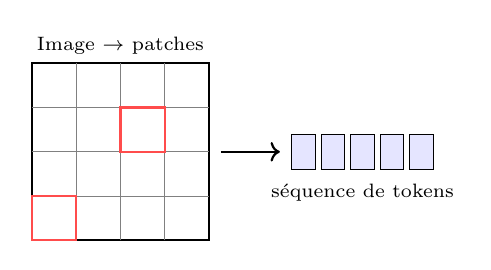
\begin{tikzpicture}[scale=0.75]
\draw[thick] (0,0) rectangle (3,3);
\foreach \x in {0.75,1.5,2.25} { \draw[gray] (\x,0) -- (\x,3); }
\foreach \y in {0.75,1.5,2.25} { \draw[gray] (0,\y) -- (3,\y); }
\draw[thick, red!70] (0,0) rectangle (0.75,0.75);
\draw[thick, red!70] (1.5,1.5) rectangle (2.25,2.25);
\node[font=\scriptsize] at (1.5,3.3) {Image $\rightarrow$ patches};

\draw[->, thick] (3.2,1.5) -- (4.2,1.5);
\foreach \i in {0,...,4} {
  \draw[fill=blue!10] (4.4+0.5*\i,1.2) rectangle (4.8+0.5*\i,1.8);
}
\node[font=\scriptsize] at (5.6,0.8) {séquence de tokens};
\end{tikzpicture}
}
\end{column}

\begin{column}{0.5\textwidth}
{\scriptsize
\setlength{\fboxsep}{4pt}
\setlength{\fboxrule}{0.8pt}
\fcolorbox{blue!70!black}{blue!10}{%
\parbox[t]{\dimexpr\linewidth-2\fboxsep-2\fboxrule\relax}{\raggedright
\textbf{Tokenisation d’image}\\
Image $X\in\mathbb{R}^{H\times W\times C}$ découpée en patches $P\times P$.\\
Nombre de tokens : $N=\frac{HW}{P^2}$.\\
Chaque patch est aplati et projeté :\\
$z_i = E\,x_i + e_i^{\text{pos}},\quad z_i\in\mathbb{R}^D$.\\
On traite ensuite $(z_1,\dots,z_N)$ comme une \textbf{séquence}.
}}
}
\end{column}
\end{columns}

\vspace{0.1cm}
\begin{center}
{\scriptsize
\textbf{Intuition :} les patches jouent le rôle de “mots” visuels ; l’attention relie des régions éloignées.
}
\end{center}
\end{frame}

\begin{frame}{Phase 3 — Auto-attention : mécanisme et coût}
\slidepurpose{Expliquer le calcul d'attention, son intérêt et son coût computationnel}{Analyse SOTA / modélisation}
\vspace*{-0.2cm}
\begin{columns}[T,onlytextwidth]
\begin{column}{0.56\textwidth}
{\scriptsize
\setlength{\fboxsep}{4pt}
\setlength{\fboxrule}{0.8pt}
\fcolorbox{blue!70!black}{blue!10}{%
\parbox[t]{\dimexpr\linewidth-2\fboxsep-2\fboxrule\relax}{\raggedright
\textbf{Auto-attention}\\
$Q=XW_Q,\quad K=XW_K,\quad V=XW_V$\\
\[
\resizebox{\linewidth}{!}{$\mathrm{Attention}(Q,K,V)=\mathrm{softmax}\!\left(\frac{QK^\top}{\sqrt{d_k}}\right)V$}
\]
$Q$ : requêtes, $K$ : clés, $V$ : valeurs.\\
Chaque token “regarde” tous les autres \textbf{(contexte global)}.
}}
\vspace{0.12cm}
\fcolorbox{red!70!black}{red!10}{%
\parbox[t]{\dimexpr\linewidth-2\fboxsep-2\fboxrule\relax}{\raggedright
\textbf{Limite de ViT}\\
Complexité quadratique : $O(N^2)$ avec $N$ tokens.\\
Pour grandes images médicales, $N$ devient très élevé $\Rightarrow$ coût prohibitif.
}}
}
\end{column}
\begin{column}{0.44\textwidth}
\centering
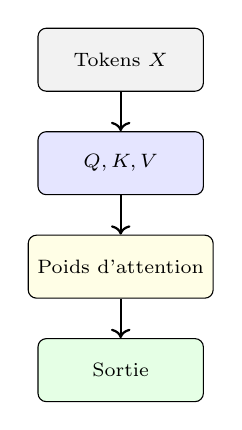
\begin{tikzpicture}[font=\scriptsize]
\node[draw, rounded corners=3pt, fill=gray!10, minimum width=2.1cm, minimum height=0.8cm] (x) {Tokens $X$};
\node[draw, rounded corners=3pt, fill=blue!10, minimum width=2.1cm, minimum height=0.8cm, below=0.5cm of x] (qkv) {$Q,K,V$};
\node[draw, rounded corners=3pt, fill=yellow!10, minimum width=2.1cm, minimum height=0.8cm, below=0.5cm of qkv] (att) {Poids d'attention};
\node[draw, rounded corners=3pt, fill=green!10, minimum width=2.1cm, minimum height=0.8cm, below=0.5cm of att] (out) {Sortie};
\draw[->, thick] (x) -- (qkv);
\draw[->, thick] (qkv) -- (att);
\draw[->, thick] (att) -- (out);
\end{tikzpicture}
\end{column}
\end{columns}
\end{frame}

\begin{frame}{Phase 3 — Swin Transformer : fenêtres et décalage}
\slidepurpose{Montrer comment Swin conserve le contexte global tout en réduisant la complexité}{Analyse SOTA / comparaison}
\vspace*{-0.2cm}
\begin{columns}[T,onlytextwidth]
\begin{column}{0.55\textwidth}
\centering
\resizebox{\linewidth}{!}{%
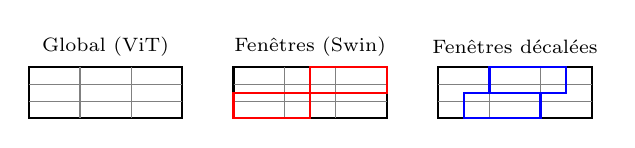
\begin{tikzpicture}[scale=0.65]
% global attention
\node[font=\scriptsize] at (1.5,3.4) {Global (ViT)};
\draw[thick] (0,2.0) rectangle (3,3.0);
\draw[gray] (1,2.0)--(1,3.0);
\draw[gray] (2,2.0)--(2,3.0);
\draw[gray] (0,2.33)--(3,2.33);
\draw[gray] (0,2.66)--(3,2.66);

% window attention
\node[font=\scriptsize] at (5.5,3.4) {Fenêtres (Swin)};
\draw[thick] (4.0,2.0) rectangle (7.0,3.0);
\draw[gray] (5.0,2.0)--(5.0,3.0);
\draw[gray] (6.0,2.0)--(6.0,3.0);
\draw[gray] (4.0,2.33)--(7.0,2.33);
\draw[gray] (4.0,2.66)--(7.0,2.66);
\draw[red, thick] (4.0,2.0) rectangle (5.5,2.5);
\draw[red, thick] (5.5,2.5) rectangle (7.0,3.0);

% shifted windows
\node[font=\scriptsize] at (9.5,3.4) {Fenêtres décalées};
\draw[thick] (8.0,2.0) rectangle (11.0,3.0);
\draw[gray] (9.0,2.0)--(9.0,3.0);
\draw[gray] (10.0,2.0)--(10.0,3.0);
\draw[gray] (8.0,2.33)--(11.0,2.33);
\draw[gray] (8.0,2.66)--(11.0,2.66);
\draw[blue, thick] (8.5,2.0) rectangle (10.0,2.5);
\draw[blue, thick] (9.0,2.5) rectangle (10.5,3.0);
\end{tikzpicture}
}
\end{column}

\begin{column}{0.45\textwidth}
{\scriptsize
\setlength{\fboxsep}{4pt}
\setlength{\fboxrule}{0.8pt}
\fcolorbox{blue!70!black}{blue!10}{%
\parbox[t]{\dimexpr\linewidth-2\fboxsep-2\fboxrule\relax}{\raggedright
\textbf{Attention par fenêtres}\\
Swin limite l’attention à des fenêtres $M\times M$ :\\
complexité $\;O\!\left(\frac{HW}{M^2}\cdot M^4\right)=O(HW\,M^2)$,\\
au lieu de $O(N^2)$ global.\\
Le \textbf{décalage} des fenêtres connecte les régions voisines.
}}
\vspace{0.12cm}
\fcolorbox{green!60!black}{green!10}{%
\parbox[t]{\dimexpr\linewidth-2\fboxsep-2\fboxrule\relax}{\raggedright
\textbf{Intérêt médical}\\
Capte des relations à longue distance tout en restant scalable.\\
Meilleure adaptation aux images haute résolution (radiographies).\\
Permet de relier des patterns subtils répartis dans l’image.
}}
}
\end{column}
\end{columns}
\end{frame}

\begin{frame}{Phase 3 — ViT/Swin : ce que fait le modèle}
\slidepurpose{Relier Transformers et radiographie thoracique en termes de bénéfices et de limites}{Analyse SOTA / pertinence applicative}
\vspace*{-0.2cm}
\begin{columns}[T,onlytextwidth]
\begin{column}{0.55\textwidth}
{\scriptsize
\setlength{\fboxsep}{4pt}
\setlength{\fboxrule}{0.8pt}
\fcolorbox{blue!70!black}{blue!10}{%
\parbox[t]{\dimexpr\linewidth-2\fboxsep-2\fboxrule\relax}{\raggedright
\textbf{Mécanisme effectif}\\
Chaque patch devient un token ; l’attention calcule l’importance \textbf{entre régions}.\\
\resizebox{\linewidth}{!}{$a_{ij}=\mathrm{softmax}\!\left(\frac{q_i k_j}{\sqrt{d}}\right),\quad \tilde z_i=\sum_j a_{ij} v_j$}\\
Le modèle combine ainsi \textbf{contexte global} et information locale.\\
Swin ajoute attention par \textbf{fenêtres} + \textbf{décalage}, puis \textbf{fusion de patches} (hiérarchie multi-échelle).
}}
}
\end{column}
\begin{column}{0.45\textwidth}
{\scriptsize
\setlength{\fboxsep}{4pt}
\setlength{\fboxrule}{0.8pt}
\fcolorbox{green!60!black}{green!10}{%
\parbox[t]{\dimexpr\linewidth-2\fboxsep-2\fboxrule\relax}{\raggedright
\textbf{Aide en imagerie médicale}\\
Relie des régions éloignées (symétrie pulmonaire, contexte global).\\
Utile pour motifs diffus et structures larges.\\
Swin reste efficace sur grandes images tout en gardant du détail.
}}
\vspace{0.12cm}
\fcolorbox{red!70!black}{red!10}{%
\parbox[t]{\dimexpr\linewidth-2\fboxsep-2\fboxrule\relax}{\raggedright
\textbf{Limites}\\
Moins d’inductif bias que les CNN $\Rightarrow$ besoin de pré-entraînement.\\
Patches trop grands $\Rightarrow$ perte de lésions fines ; trop petits $\Rightarrow$ coût élevé.\\
Attention peut suivre des corrélats non pathologiques.
}}
}
\end{column}
\end{columns}
\end{frame}

% ==================================================
% PHASE 4 — Grad-CAM
% ==================================================
\subsection{Phase 4 — Confiance et explicabilité}

\begin{frame}{Phase 4 — Grad-CAM : principe et formulation}
\slidepurpose{Définir l'outil d'explicabilité utilisé pour interpréter les prédictions}{Analyse SOTA / évaluation interprétable}
\vspace*{-0.2cm}
\begin{columns}[T,onlytextwidth]
\begin{column}{0.55\textwidth}
{\scriptsize
\setlength{\fboxsep}{4pt}
\setlength{\fboxrule}{0.8pt}
\fcolorbox{red!70!black}{red!10}{%
\parbox[t]{\dimexpr\linewidth-2\fboxsep-2\fboxrule\relax}{\raggedright
\textbf{Idée}\\
Grad-CAM met en évidence \textbf{où} le réseau “regarde” pour une classe donnée.\\
On utilise les gradients du score $y^c$ par rapport aux cartes $A^k$.
}}
\vspace{0.12cm}
\fcolorbox{orange!80!black}{yellow!15}{%
\parbox[t]{\dimexpr\linewidth-2\fboxsep-2\fboxrule\relax}{\raggedright
\textbf{Formules}\\
Poids d’importance :\\
\resizebox{.6\linewidth}{!}{$\alpha_k^c=\frac{1}{Z}\sum_i\sum_j \frac{\partial y^c}{\partial A^k_{ij}}$}\\
Carte Grad-CAM :\\
\resizebox{.6\linewidth}{!}{$L_{\text{Grad-CAM}}^c=\mathrm{ReLU}\!\left(\sum_k \alpha_k^c A^k\right)$}
}}
}
\end{column}

\begin{column}{0.45\textwidth}
{\scriptsize
\setlength{\fboxsep}{4pt}
\setlength{\fboxrule}{0.8pt}
\fcolorbox{blue!70!black}{blue!10}{%
\parbox[t]{\dimexpr\linewidth-2\fboxsep-2\fboxrule\relax}{\raggedright
\textbf{Interprétation}\\
$A^k$ : carte de features de la dernière couche conv.\\
$\alpha_k^c$ : contribution de la carte $k$ à la classe $c$.\\
ReLU conserve les contributions positives.\\
Le modèle donne \textbf{“quoi”}, Grad-CAM suggère \textbf{“où”}.
}}
}
\end{column}
\end{columns}
\end{frame}

\begin{frame}{Phase 4 — Grad-CAM : schéma de génération}
\slidepurpose{Visualiser le pipeline complet de production d'une heatmap explicative}{Analyse SOTA / évaluation interprétable}
\vspace*{-0.2cm}
\centering
\resizebox{\textwidth}{!}{%
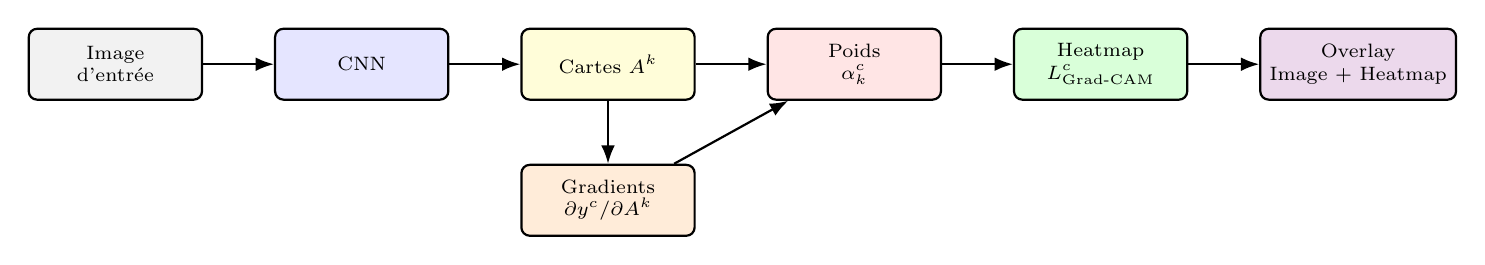
\begin{tikzpicture}[
    >=Latex,
    font=\scriptsize,
    box/.style={draw, rounded corners=3pt, align=center, thick, minimum width=2.2cm, minimum height=0.9cm}
]
\node[box, fill=gray!10] (img) {Image\\d’entrée};
\node[box, fill=blue!10, right=0.9cm of img] (cnn) {CNN};
\node[box, fill=yellow!15, right=0.9cm of cnn] (feat) {Cartes $A^k$};
\node[box, fill=orange!15, below=0.8cm of feat] (grad) {Gradients\\$\partial y^c/\partial A^k$};
\node[box, fill=red!10, right=0.9cm of feat] (weights) {Poids\\$\alpha_k^c$};
\node[box, fill=green!15, right=0.9cm of weights] (heat) {Heatmap\\$L_{\text{Grad-CAM}}^c$};
\node[box, fill=violet!15, right=0.9cm of heat] (overlay) {Overlay\\Image + Heatmap};

\draw[->, thick] (img) -- (cnn);
\draw[->, thick] (cnn) -- (feat);
\draw[->, thick] (feat) -- (weights);
\draw[->, thick] (weights) -- (heat);
\draw[->, thick] (heat) -- (overlay);
\draw[->, thick] (feat) -- (grad);
\draw[->, thick] (grad) -- (weights);
\end{tikzpicture}
}

\vspace{0.12cm}
{\scriptsize
\textbf{Lecture :} l’overlay montre les régions activées associées à la classe prédite.
}
\end{frame}

\begin{frame}{Phase 4 — Grad-CAM : ce que ça aide (et ce que ça n’aide pas)}
\slidepurpose{Préciser l'utilité clinique réelle de Grad-CAM et ses limites méthodologiques}{Analyse SOTA / validation critique}
\vspace*{-0.2cm}
\begin{columns}[T,onlytextwidth]
\begin{column}{0.55\textwidth}
{\scriptsize
\setlength{\fboxsep}{4pt}
\setlength{\fboxrule}{0.8pt}
\fcolorbox{green!60!black}{green!10}{%
\parbox[t]{\dimexpr\linewidth-2\fboxsep-2\fboxrule\relax}{\raggedright
\textbf{Ce que Grad-CAM apporte}\\
Explication \textbf{post-hoc} : montre quelles zones augmentent le score $y^c$.\\
Ne modifie pas la prédiction, mais \textbf{guide l’analyse} (triage, relecture).\\
Utile pour repérer des biais (texte, marqueurs, position).\\
Permet d’aligner le modèle avec l’expertise clinique.
}}
}
\end{column}
\begin{column}{0.45\textwidth}
{\scriptsize
\setlength{\fboxsep}{4pt}
\setlength{\fboxrule}{0.8pt}
\fcolorbox{red!70!black}{red!10}{%
\parbox[t]{\dimexpr\linewidth-2\fboxsep-2\fboxrule\relax}{\raggedright
\textbf{Ce que Grad-CAM ne garantit pas}\\
Carte \textbf{grossière} (résolution = stride de la dernière couche).\\
Importance $\neq$ causalité ; une heatmap “plausible” peut être trompeuse.\\
Sensibilité à la couche choisie, au prétraitement et au bruit.\\
\textbf{Interprétabilité = aide}, pas preuve diagnostique.
}}
}
\end{column}
\end{columns}
\end{frame}

\section{Solution proposée}
\subsection{Architecture et conception}

\begin{frame}[t]{Solution proposée — Étape 0 : vue d'ensemble}
\slidepurpose{Présenter la logique globale du modèle avant le détail des étapes}{Conception de la solution}
\vspace*{-0.18cm}
\begin{columns}[T,onlytextwidth]
\begin{column}{0.56\textwidth}
\scriptsize
\setlength{\abovedisplayskip}{3pt}
\setlength{\belowdisplayskip}{3pt}
\begin{block}{Principe et formule globale}
MedFusionNet combine deux lectures d'une même radiographie :
\begin{itemize}
\setlength{\itemsep}{0.15em}
\item une branche \textbf{CNN} pour les indices locaux : contours, textures, petites opacités ;
\item une branche \textbf{Swin} pour le contexte global : symétrie thoracique, bilatéralité, cohérence anatomique ;
\item une \textbf{fusion guidée} qui pondère automatiquement les deux branches.
\end{itemize}
\textbf{Chaîne mathématique.}
\[
\begin{aligned}
\tilde X &= T(X)\\
F_c &= \Phi_c(\tilde X), \qquad F_s = \Phi_s(\tilde X)
\end{aligned}
\]
\[
\begin{aligned}
g &= \sigma\!\big(W_g[\mathrm{GAP}(F_c),\mathrm{GAP}(F_s)] + b_g\big)\\
F &= g\odot F_c + (1-g)\odot F_s
\end{aligned}
\]
La sortie finale vérifie \(\Psi(F)=(p,L^c,u)\) : score $p$, heatmap $L^c$, incertitude $u$.
\end{block}
\end{column}
\begin{column}{0.44\textwidth}
\solutionfigure{solution_step_00_overview.png}{Vue d'ensemble du pipeline complet}
\end{column}
\end{columns}
\end{frame}

\subsection{Pipeline détaillé}

\begin{frame}[t]{Solution proposée — Étape 1 : échantillon d'entrée}
\slidepurpose{Définir la donnée d'entrée et ce qu'elle contient avant tout calcul}{Conception détaillée}
\vspace*{-0.18cm}
\begin{columns}[T,onlytextwidth]
\begin{column}{0.56\textwidth}
\scriptsize
\setlength{\abovedisplayskip}{3pt}
\setlength{\belowdisplayskip}{3pt}
\begin{block}{Image et variabilité}
Une radiographie thoracique est modélisée par :
\[
X\in\mathbb{R}^{H\times W}
\]
\noindent avec une étiquette binaire :
\[
\begin{cases}
y=1 & \text{pneumonie}\\
y=0 & \text{normal ou autre classe négative}
\end{cases}
\]
\textbf{Pourquoi l'entrée est difficile.}
L'image brute contient à la fois le signal clinique et des facteurs parasites :
\begin{itemize}
\setlength{\itemsep}{0.15em}
\item variations d'intensité et de contraste selon l'appareil ;
\item bruit, annotations, câbles et autres artefacts ;
\item cadrage, résolution et structures normales parfois trompeuses.
\end{itemize}
\textbf{Exemple :} deux clichés de même classe peuvent avoir un contraste ou un centrage très différents ; le modèle doit ignorer cette variabilité non pathologique.
\end{block}
\end{column}
\begin{column}{0.44\textwidth}
\solutionfigure{solution_step_01_input_sample.png}{Échantillon brut provenant du dataset}
\end{column}
\end{columns}
\end{frame}

\begin{frame}[t]{Solution proposée — Étape 2 : prétraitement}
\slidepurpose{Standardiser l'image avant son entrée dans les deux branches du modèle}{Développement / préparation des données}
\vspace*{-0.18cm}
\begin{columns}[T,onlytextwidth]
\begin{column}{0.56\textwidth}
\scriptsize
\setlength{\abovedisplayskip}{3pt}
\setlength{\belowdisplayskip}{3pt}
\begin{block}{Transformation}
Le prétraitement applique une chaîne de standardisation :
\[
\tilde X=T(X)=A\big(R(N(X))\big)
\]
\noindent où $N$ normalise les intensités, $R$ redimensionne et $A$ peut améliorer localement le contraste.
\end{block}
\begin{block}{Ce que la donnée devient}
\[
\text{normalisation :}\qquad X_{norm}=\frac{X-\mu}{\sigma}
\]
\[
\begin{aligned}
\text{redimensionnement :}\qquad
X&\in\mathbb{R}^{H\times W}\\
&\longrightarrow \tilde X\in\mathbb{R}^{H_0\times W_0}
\end{aligned}
\]
\textbf{Exemple :} $1024\times1024 \rightarrow 384\times384$. Cette étape réduit le coût mémoire, homogénéise les entrées et diminue le risque que le modèle prenne une différence d'acquisition pour une pneumonie.
\end{block}
\end{column}
\begin{column}{0.44\textwidth}
\solutionfigure{solution_step_02_preprocessing.png}{Image après normalisation et redimensionnement}
\end{column}
\end{columns}
\end{frame}

\begin{frame}[t]{Solution proposée — Étape 3 : branche CNN locale}
\slidepurpose{Extraire les motifs fins et localisés par une lecture convolutive}{Modélisation de la branche locale}
\vspace*{-0.18cm}
\begin{columns}[T,onlytextwidth]
\begin{column}{0.56\textwidth}
\scriptsize
\setlength{\abovedisplayskip}{3pt}
\setlength{\belowdisplayskip}{3pt}
\begin{block}{Lecture locale par CNN}
La branche locale produit :
\[
F_c=\Phi_c(\tilde X)\in\mathbb{R}^{H'\times W'\times C_c}
\]
\noindent Une convolution applique un filtre sur un voisinage restreint :
\[
F^{(\ell)}_{i,j,c'}=\sum_{u,v,c}W^{(\ell)}_{u,v,c,c'}\,F^{(\ell-1)}_{i+u,j+v,c}+b^{(\ell)}_{c'}
\]
\textbf{Ce que la branche voit réellement.}
\begin{itemize}
\setlength{\itemsep}{0.15em}
\item bords pleuraux, côtes, contours pulmonaires ;
\item textures diffuses ou focales ;
\item petites consolidations et opacités locales ;
\item transitions fines entre tissu sain et tissu suspect.
\end{itemize}
\textbf{Exemple :} une opacité basale discrète peut être amplifiée par la comparaison locale entre intensités voisines.
\end{block}
\end{column}
\begin{column}{0.44\textwidth}
\solutionfigure{solution_step_03_cnn_local.png}{Représentation locale extraite par la branche CNN}
\end{column}
\end{columns}
\end{frame}

\begin{frame}[t]{Solution proposée — Étape 4 : branche Swin globale}
\slidepurpose{Extraire une représentation de contexte capable de relier des régions éloignées}{Modélisation de la branche globale}
\vspace*{-0.18cm}
\begin{columns}[T,onlytextwidth]
\begin{column}{0.56\textwidth}
\scriptsize
\setlength{\abovedisplayskip}{3pt}
\setlength{\belowdisplayskip}{3pt}
\begin{block}{Lecture globale par Swin}
L'image prétraitée est découpée en patches puis projetée :
\[
z_i = E\,x_i + e_i^{pos}
\]
\noindent La branche globale calcule ensuite :
\[
F_s=\Phi_s(\tilde X)\in\mathbb{R}^{H'\times W'\times C_s}
\]
\[
Q=XW_Q,\quad K=XW_K,\quad V=XW_V
\]
\[
\mathrm{Attention}(Q,K,V)=\mathrm{softmax}\!\left(\frac{QK^\top}{\sqrt{d_k}}\right)V
\]
Dans Swin, cette attention est calculée par fenêtres, puis les fenêtres sont décalées pour reconnecter les régions voisines.
\textbf{Ce que la branche globale apporte.}
Elle relie des zones éloignées : apex, bases, hémithorax droit/gauche, médiastin. Si une anomalie n'a de sens que par sa \textbf{distribution spatiale}, Swin la capture mieux qu'un CNN purement local.
\end{block}
\end{column}
\begin{column}{0.44\textwidth}
\solutionfigure{solution_step_04_swin_global.png}{Représentation globale extraite par la branche Swin}
\end{column}
\end{columns}
\end{frame}

\begin{frame}[t]{Solution proposée — Étape 5 : fusion guidée}
\slidepurpose{Combiner les indices locaux et globaux sans imposer un poids fixe à chaque branche}{Conception du coeur de fusion}
\vspace*{-0.18cm}
\begin{columns}[T,onlytextwidth]
\begin{column}{0.56\textwidth}
\scriptsize
\setlength{\abovedisplayskip}{3pt}
\setlength{\belowdisplayskip}{3pt}
\begin{block}{Porte de fusion et interprétation}
On résume d'abord chaque branche par un vecteur global :
\[
\bar F_c=\mathrm{GAP}(F_c),\qquad \bar F_s=\mathrm{GAP}(F_s)
\]
\noindent Puis on apprend un coefficient de fusion :
\[
g=\sigma\!\left(W_g[\bar F_c,\bar F_s]+b_g\right)
\]
\[
F = g\odot F_c + (1-g)\odot F_s
\]
Si $g\approx 1$, le modèle privilégie l'indice local ; si $g\approx 0$, il privilégie le contexte global.
\textbf{Exemples.}
\textbf{Exemple 1 :} foyer net et compact $\Rightarrow g\approx 0.8$.\\
\textbf{Exemple 2 :} atteinte diffuse ou bilatérale $\Rightarrow g\approx 0.3$.\\[0.15em]
La fusion n'est donc pas une moyenne fixe : elle s'adapte à la structure réelle de l'image.
\end{block}
\end{column}
\begin{column}{0.44\textwidth}
\solutionfigure{solution_step_05_gated_fusion.png}{Fusion adaptative entre la branche locale et la branche globale}
\end{column}
\end{columns}
\end{frame}

\begin{frame}[t]{Solution proposée — Étape 6 : classification}
\slidepurpose{Transformer la représentation fusionnée en probabilité de pneumonie}{Tête de décision}
\vspace*{-0.18cm}
\begin{columns}[T,onlytextwidth]
\begin{column}{0.56\textwidth}
\scriptsize
\setlength{\abovedisplayskip}{3pt}
\setlength{\belowdisplayskip}{3pt}
\begin{block}{Score de classe}
La représentation fusionnée est condensée en un vecteur :
\[
z=\mathrm{GAP}(F)
\]
\noindent puis convertie en probabilité :
\[
p(y=1|X)=\sigma(w^\top z+b)
\]
\end{block}
\begin{block}{Décision pratique}
Avec un seuil $\tau$ :
\[
\hat y =
\begin{cases}
1 & \text{si } p(y=1|X)\ge \tau\\
0 & \text{sinon}
\end{cases}
\]
\textbf{Exemple :} si $p=0.91$ et $\tau=0.5$, la prédiction est positive avec une forte marge. Si $p=0.54$, la décision reste positive mais devient fragile : elle doit être lue avec la heatmap et l'incertitude.
\end{block}
\end{column}
\begin{column}{0.44\textwidth}
\solutionfigure{solution_step_06_classification.png}{Passage de la représentation fusionnée au score de classe}
\end{column}
\end{columns}
\end{frame}

\begin{frame}[t]{Solution proposée — Étape 7 : localisation et incertitude}
\slidepurpose{Produire une explication spatiale et mesurer la fiabilité de la décision}{Sorties interprétables}
\vspace*{-0.18cm}
\begin{columns}[T,onlytextwidth]
\begin{column}{0.56\textwidth}
\footnotesize
\setlength{\abovedisplayskip}{3pt}
\setlength{\belowdisplayskip}{3pt}
\begin{block}{Localisation et incertitude}
À partir des cartes finales $A^k$ :
\[
\alpha_k^c=\frac{1}{Z}\sum_i\sum_j \frac{\partial y^c}{\partial A^k_{ij}}
\]
\[
L^c=\mathrm{ReLU}\!\left(\sum_k \alpha_k^c A^k\right)
\]
La heatmap montre \textbf{où} le modèle a trouvé des indices pour la classe prédite.
\textbf{Incertitude.}
En répétant plusieurs passes avec dropout actif :
\[
u=\mathrm{Var}_t(p_t)
\]
\textbf{Exemple :} si $p_t=\{0.87,0.88,0.89\}$, la variance est faible ; si $p_t=\{0.42,0.81,0.57\}$, la décision est instable et doit être relue.
\end{block}
\end{column}
\begin{column}{0.44\textwidth}
\solutionfigure{solution_step_07_localization_uncertainty.png}{Heatmap explicative et estimation d'incertitude}
\end{column}
\end{columns}
\end{frame}

\begin{frame}[t]{Solution proposée — Étape 8 : apprentissage}
\slidepurpose{Définir exactement ce qui est optimisé pendant l'entraînement}{Développement / entraînement}
\vspace*{-0.18cm}
\begin{columns}[T,onlytextwidth]
\begin{column}{0.56\textwidth}
\footnotesize
\setlength{\abovedisplayskip}{3pt}
\setlength{\belowdisplayskip}{3pt}
\begin{block}{Fonction objectif}
\[
\mathcal{L}=
\mathcal{L}_{cls}
\;+\;
\lambda_1\mathcal{L}_{loc}
\;+\;
\lambda_2\mathcal{L}_{cons}
\;+\;
\lambda_3\mathcal{L}_{cal}
\]
\end{block}
\begin{block}{Sens de chaque terme}
\defitem{$\mathcal{L}_{cls}$}{apprendre la bonne classe.}
\defitem{$\mathcal{L}_{loc}$}{contraindre la heatmap à rester cliniquement plausible.}
\defitem{$\mathcal{L}_{cons}$}{garder une prédiction stable sous augmentation.}
\defitem{$\mathcal{L}_{cal}$}{mieux aligner confiance prédite et fréquence réelle d'erreur.}
\textbf{Exemple :} sur un dataset déséquilibré, $\mathcal{L}_{cls}$ peut être une Focal Loss afin de mieux traiter les cas rares ou difficiles.
\end{block}
\end{column}
\begin{column}{0.44\textwidth}
\solutionfigure{solution_step_08_training_objective.png}{Schéma de la perte totale et de ses composantes}
\end{column}
\end{columns}
\end{frame}

\begin{frame}[t]{Solution proposée — Étape 9 : sortie clinique}
\slidepurpose{Montrer comment les sorties du modèle deviennent une aide concrète pour le workflow médical}{Validation métier / déploiement}
\vspace*{-0.18cm}
\begin{columns}[T,onlytextwidth]
\begin{column}{0.56\textwidth}
\footnotesize
\setlength{\abovedisplayskip}{3pt}
\setlength{\belowdisplayskip}{3pt}
\begin{block}{Sortie exploitable pour le clinicien}
Pour une image $X$, le modèle renvoie :
\[
\big(p(y=1|X),\,L^c,\,u\big)
\]
soit un score de pneumonie, une heatmap explicative et une estimation d'incertitude.
\textbf{Comment cela aide le clinicien.}
\begin{itemize}
\setlength{\itemsep}{0.15em}
\item score élevé + faible incertitude : cas à prioriser ;
\item score modéré + incertitude élevée : revue humaine prioritaire ;
\item score faible + faible incertitude : cas probablement normal.
\end{itemize}
\textbf{Limite :} une heatmap plausible reste un support de lecture, pas une preuve diagnostique.
\end{block}
\end{column}
\begin{column}{0.44\textwidth}
\solutionfigure{solution_step_09_clinical_output.png}{Sortie finale utilisable par le clinicien}
\end{column}
\end{columns}
\end{frame}

\section{Résultats et Finalisation}

\begin{frame}{Résultats obtenus}
\slidepurpose{Présenter les indicateurs de performance et leur interprétation métier}{Évaluation finale}
    \begin{columns}
        \begin{column}{0.5\textwidth}
            \begin{block}{Métriques de Performance}
                \begin{itemize}
                    \item \textbf{Précision (Accuracy) :} $\approx$ 92\%
                    \item \textbf{Sensibilité (Recall) :} 94\%
                    \item \textbf{AUC-ROC :} 0.96
                \end{itemize}
            \end{block}
        \end{column}
        \begin{column}{0.5\textwidth}
            \begin{itemize}
                \item Réduction significative des faux négatifs.
                \item Génération de \textbf{Grad-CAM} fonctionnelle pour valider les zones d'intérêt.
            \end{itemize}
        \end{column}
    \end{columns}
\end{frame}

\begin{frame}{Mots clés}
\slidepurpose{Synthétiser les thèmes techniques majeurs couverts par le document}{Clôture documentaire}
    \begin{center}
        \fbox{Intelligence Artificielle} \quad \fbox{Deep Learning} \quad \fbox{Vision par Ordinateur} \\
        \vspace{0.5cm}
        \fbox{Radiographie Thoracique (CXR)} \quad \fbox{Pneumonie} \quad \fbox{CNN / Transformers} \\
        \vspace{0.5cm}
        \fbox{Transfer Learning} \quad \fbox{Interprétabilité (Grad-CAM)}
    \end{center}
\end{frame}

\appendix
\section{Annexes}
\subsection{Références techniques}

\begin{frame}{Annexe A — Convolution, stride et pooling}
\slidepurpose{Définir les opérations de base des CNN utilisées dans les architectures étudiées}{Annexe technique}
\small
\begin{columns}[T,onlytextwidth]
\begin{column}{0.48\textwidth}
\begin{block}{Definitions}
\defitem{Convolution $k\times k$}{Filtre local glissant sur l'image ou sur une carte de features.}
\defitem{Stride $s$}{Pas de déplacement du filtre ; quand $s$ augmente, la résolution baisse plus vite.}
\defitem{Padding}{Bordure ajoutée pour contrôler la taille de sortie.}
\defitem{MaxPool}{Conserve la plus forte activation dans une fenêtre locale.}
\defitem{AvgPool}{Remplace une fenêtre locale par sa moyenne.}
\end{block}
\end{column}
\begin{column}{0.48\textwidth}
\begin{block}{Formules utiles}
\[
Y_{i,j,c'}=\sum_{u,v,c}W_{u,v,c,c'}X_{i+u,j+v,c}+b_{c'}
\]
\[
H_{out}=\left\lfloor \frac{H+2p-k}{s}\right\rfloor +1
\]
\end{block}
\begin{block}{Intuition}
Les convolutions extraient des motifs locaux. Le pooling résume l'information et réduit la taille spatiale pour rendre le calcul plus efficace.
\end{block}
\end{column}
\end{columns}
\end{frame}

\begin{frame}{Annexe B — BN, ReLU, bottleneck et connexions}
\slidepurpose{Clarifier les briques de stabilisation et d'efficacité citées dans DenseNet et EfficientNet}{Annexe technique}
\small
\begin{columns}[T,onlytextwidth]
\begin{column}{0.48\textwidth}
\begin{block}{Stabilisation}
\defitem{BN}{Normalise les activations d'un mini-batch pour stabiliser et accélérer l'entraînement.}
\defitem{ReLU}{Garde les valeurs positives et annule les négatives, ce qui introduit une non-linéarité simple.}
\defitem{Skip connection}{Réinjecte une information plus tôt dans le réseau pour faciliter le gradient.}
\end{block}
\end{column}
\begin{column}{0.48\textwidth}
\begin{block}{Efficacité}
\defitem{Bottleneck}{Réduit les canaux avant une opération coûteuse, puis projette de nouveau si besoin.}
\defitem{Growth rate $k$}{Nombre de nouveaux canaux ajoutés par chaque couche dense.}
\defitem{SE}{Mécanisme qui ré-pondère les canaux selon leur importance.}
\defitem{Fused-MBConv}{Version simplifiée de MBConv, souvent plus rapide à entraîner sur GPU dans les premiers étages.}
\end{block}
\end{column}
\end{columns}
\end{frame}

\begin{frame}{Annexe C — DenseNet et MBConv}
\slidepurpose{Reprendre proprement les blocs spécifiques les plus utilisés dans l'analyse SOTA}{Annexe technique}
\small
\begin{columns}[T,onlytextwidth]
\begin{column}{0.48\textwidth}
\begin{block}{Bloc dense}
DenseNet concatène les sorties précédentes au lieu de simplement les additionner.
\[
x_\ell = H_\ell([x_0,\dots,x_{\ell-1}])
\]
Cela favorise la réutilisation des features et un meilleur flux de gradient.
\end{block}
\end{column}
\begin{column}{0.48\textwidth}
\begin{block}{MBConv}
MBConv combine :
\begin{itemize}
\setlength{\itemsep}{0.35em}
\item une expansion $1\times1$,
\item une convolution depthwise,
\item un module SE,
\item une projection finale $1\times1$.
\end{itemize}
L'objectif est d'obtenir une bonne expressivité à coût réduit.
\end{block}
\end{column}
\end{columns}
\end{frame}

\begin{frame}{Annexe D — Vocabulaire Transformer}
\slidepurpose{Définir les notions de patchs, tokens et embeddings utilisées dans ViT et Swin}{Annexe technique}
\small
\begin{columns}[T,onlytextwidth]
\begin{column}{0.48\textwidth}
\begin{block}{Definitions}
\defitem{Patch}{Sous-image locale de taille $P\times P$.}
\defitem{Token}{Vecteur obtenu après projection d'un patch.}
\defitem{Embedding}{Représentation vectorielle dense envoyée dans le Transformer.}
\defitem{Encodage positionnel}{Information ajoutée pour conserver l'ordre spatial des patches.}
\end{block}
\end{column}
\begin{column}{0.48\textwidth}
\begin{block}{Formule de tokenisation}
\[
N=\frac{HW}{P^2},\qquad z_i = E\,x_i + e_i^{pos}
\]
\end{block}
\begin{block}{Intuition}
Le Transformer traite l'image comme une séquence de morceaux visuels, de la même façon qu'un modèle de langage traite une phrase comme une séquence de mots.
\end{block}
\end{column}
\end{columns}
\end{frame}

\begin{frame}{Annexe E — Attention et Swin}
\slidepurpose{Détailler le calcul d'attention et la logique des fenêtres décalées de Swin}{Annexe technique}
\small
\begin{columns}[T,onlytextwidth]
\begin{column}{0.48\textwidth}
\begin{block}{Attention}
\[
Q=XW_Q,\quad K=XW_K,\quad V=XW_V
\]
\[
\resizebox{0.95\linewidth}{!}{$\mathrm{Attention}(Q,K,V)=\mathrm{softmax}\!\left(\frac{QK^\top}{\sqrt{d_k}}\right)V$}
\]
\defitem{$Q$}{Ce que le token courant cherche.}
\defitem{$K$}{Ce que les autres tokens proposent pour être reliés à lui.}
\defitem{$V$}{L'information qui sera effectivement transmise.}
\end{block}
\end{column}
\begin{column}{0.48\textwidth}
\begin{block}{Pourquoi Swin}
\defitem{Fenêtre}{Sous-ensemble local de tokens traité ensemble.}
\defitem{Fenêtres décalées}{Décalage d'une couche à la suivante pour reconnecter des zones voisines.}
\defitem{Bénéfice}{Réduire le coût du contexte global tout en conservant des interactions spatiales utiles.}
\end{block}
\begin{block}{Complexité}
L'attention globale est quadratique en nombre de tokens. Swin réduit ce coût en limitant l'attention à des fenêtres locales.
\end{block}
\end{column}
\end{columns}
\end{frame}

\begin{frame}{Annexe F — Entraînement complémentaire}
\slidepurpose{Définir les notions d'entraînement mentionnées sans détail dans la solution proposée}{Annexe technique}
\small
\begin{columns}[T,onlytextwidth]
\begin{column}{0.48\textwidth}
\begin{block}{Concepts de base}
\defitem{Transfer learning}{Réutiliser un modèle pré-entraîné puis l'adapter à la radiographie thoracique.}
\defitem{Augmentation}{Modifier l'image pendant l'entraînement pour rendre le modèle plus robuste.}
\defitem{Pseudo-masque}{Zone approximative utilisée comme supervision faible quand on n'a pas d'annotation pixel exacte.}
\defitem{Logit}{Score brut avant application de la sigmoïde ou du softmax.}
\end{block}
\end{column}
\begin{column}{0.48\textwidth}
\begin{block}{Pourquoi c'est utile}
Ces mécanismes servent à :
\begin{itemize}
\setlength{\itemsep}{0.35em}
\item mieux généraliser,
\item réduire la dépendance à un seul centre hospitalier,
\item exploiter des annotations incomplètes,
\item stabiliser l'apprentissage quand les données sont déséquilibrées.
\end{itemize}
\end{block}
\end{column}
\end{columns}
\end{frame}

\begin{frame}{Annexe G — Pertes et calibration}
\slidepurpose{Définir les fonctions objectif et la notion de confiance calibrée}{Annexe technique}
\small
\begin{columns}[T,onlytextwidth]
\begin{column}{0.5\textwidth}
\begin{block}{Fonctions de perte}
\defitem{BCE}{Binary Cross-Entropy, perte standard de classification binaire.}
\defitem{Focal loss}{Version de BCE qui met davantage l'accent sur les exemples difficiles ou rares.}
\defitem{$\mathcal{L}_{cons}$}{Impose des sorties proches pour deux vues augmentées d'une même image.}
\defitem{$\mathcal{L}_{loc}$}{Contraint la carte explicative à rester cohérente avec une zone plausible.}
\end{block}
\[
\mathcal{L}_{BCE}=-(y\log p +(1-y)\log(1-p))
\]
\end{column}
\begin{column}{0.5\textwidth}
\begin{block}{Calibration}
\defitem{Calibration}{Une probabilité 0.8 devrait correspondre à environ 80\% de prédictions correctes.}
\defitem{Temperature scaling}{Correction post-hoc des logits par un scalaire de température.}
\defitem{ECE}{Mesure l'écart entre confiance moyenne et précision réelle.}
\end{block}
\[
\mathrm{ECE}=\sum_{m=1}^{M}\frac{|B_m|}{n}\left|\mathrm{acc}(B_m)-\mathrm{conf}(B_m)\right|
\]
\end{column}
\end{columns}
\end{frame}

\begin{frame}{Annexe H — Fusion, explicabilité et incertitude}
\slidepurpose{Documenter les sorties avancées de la solution proposée}{Annexe technique}
\small
\begin{columns}[T,onlytextwidth]
\begin{column}{0.48\textwidth}
\begin{block}{Fusion et gating}
Le gating apprend le poids relatif des branches locale et globale.
\[
g=\sigma(W_g[\mathrm{GAP}(F_c),\mathrm{GAP}(F_s)])
\]
\[
F=g\odot F_c + (1-g)\odot F_s
\]
Si $g$ est grand, la branche CNN domine ; sinon la branche Swin domine.
\end{block}
\end{column}
\begin{column}{0.48\textwidth}
\begin{block}{Explicabilité et confiance}
\defitem{Grad-CAM}{Carte visuelle des zones qui contribuent positivement au score choisi.}
\defitem{MC-Dropout}{Plusieurs passes avec dropout actif à l'inférence pour estimer l'incertitude.}
\defitem{Variance prédictive}{Plus elle est grande, moins la décision est fiable.}
\[
u=\mathrm{Var}_{t}(p_t)
\]
\end{block}
\end{column}
\end{columns}
\end{frame}

\begin{frame}{Annexe I — Metriques d'evaluation}
\slidepurpose{Définir précisément les mesures de performance et leur lecture clinique}{Annexe technique}
\small
\begin{columns}[T,onlytextwidth]
\begin{column}{0.48\textwidth}
\begin{block}{Definitions}
\defitem{Accuracy}{Proportion totale de prédictions correctes.}
\defitem{Recall / Sensibilité}{Capacité à retrouver les cas positifs.}
\defitem{Spécificité}{Capacité à rejeter les cas négatifs.}
\defitem{AUC-ROC}{Qualité de séparation entre classes quand on fait varier le seuil.}
\defitem{Faux positif}{Cas sain déclaré malade.}
\defitem{Faux négatif}{Cas malade déclaré sain.}
\end{block}
\end{column}
\begin{column}{0.48\textwidth}
\begin{block}{Formules}
\[
\resizebox{0.92\linewidth}{!}{$\mathrm{Recall}=\frac{TP}{TP+FN},\qquad
\mathrm{Specificite}=\frac{TN}{TN+FP}$}
\]
\[
\resizebox{0.82\linewidth}{!}{$\mathrm{Accuracy}=\frac{TP+TN}{TP+TN+FP+FN}$}
\]
\end{block}
\begin{block}{Lecture en contexte médical}
En dépistage de pneumonie, réduire les faux négatifs est souvent prioritaire : manquer un cas pathologique est généralement plus grave que sur-appeler un cas douteux.
\end{block}
\end{column}
\end{columns}
\end{frame}

\end{document}
